\chapter{Results}
\label{ch:results}

% sections
% 1 qualitative analysis (added by me)
% 2 setup
% 3 acquisition params
% 4 data treatment



% intro to results
This chapter presents the results of the thesis.
The results are divided into four parts: qualitative analysis of the spectra, characterization of the setup, optimization of the acquisition parameters, and data treatment.
As seen in the SE images presented in \cref{method:SE_images}, the areas chosen for the analysis are homogeneous and relatively clean.
Scratched areas on the GaSb specimen are shown in \cref{fig:SE_images:GaSb} panel (b), where some spectra were acquired, but not included in the results of this thesis.
% TODO discuss: the scratched areas behaved as expected, yielding poorer results than the homogeneous areas. ISO etc.



% 1 qualitative analysis
\section{Qualitative analysis}
\label{results:qualitative_analysis}

Here, an overview of the spectra is presented, where some characteristics and artifacts are identified, before addressing the setup parameters in \cref{results:setup}, acquisition parameters in \cref{results:acquisition_parameters}, and quantification results in \cref{results:data_treatment}.
General plots of the spectra are given in \cref{fig:results:overviewGaSb_withArtifacts,fig:results:GaSb_voltages,fig:results:GaAs_voltages}.



% figures/results/spectrum_overview.pdf
\begin{figure}[hbtp]
    \centering
    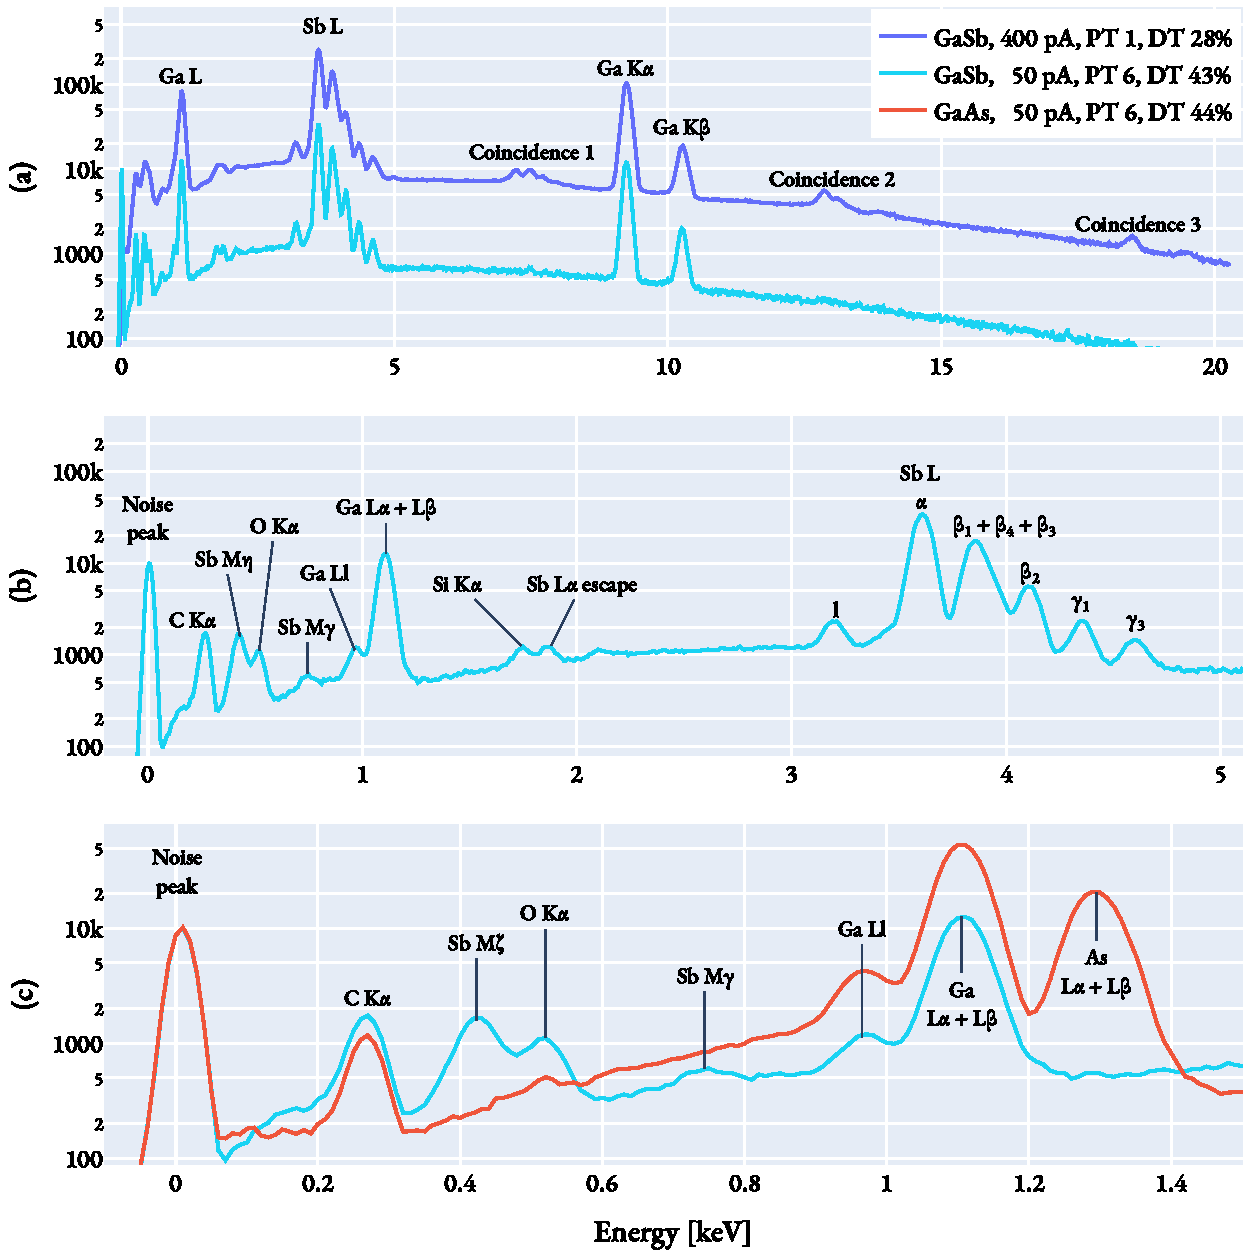
\includegraphics[width=0.99\linewidth]{figures/results/spectrum_overviews.pdf}
    \caption{
        Overview of the GaSb spectra.
        The blue line in panel (a) have lower resolution and more artifacts than the light blue line.
        The light blue line is plotted in panel (b) over a shorter energy range, and with peaks annotated.
        Panel (c) show the light blue line on an even shorter energy range, with the GaAs spectrum in red for reference.
        All three spectra are acquired with 30 kV.
    }
    \label{fig:results:overviewGaSb_withArtifacts}
\end{figure}


% figures/results/GaAs_voltages.pdf
\begin{figure}[hbtp]
    \centering
    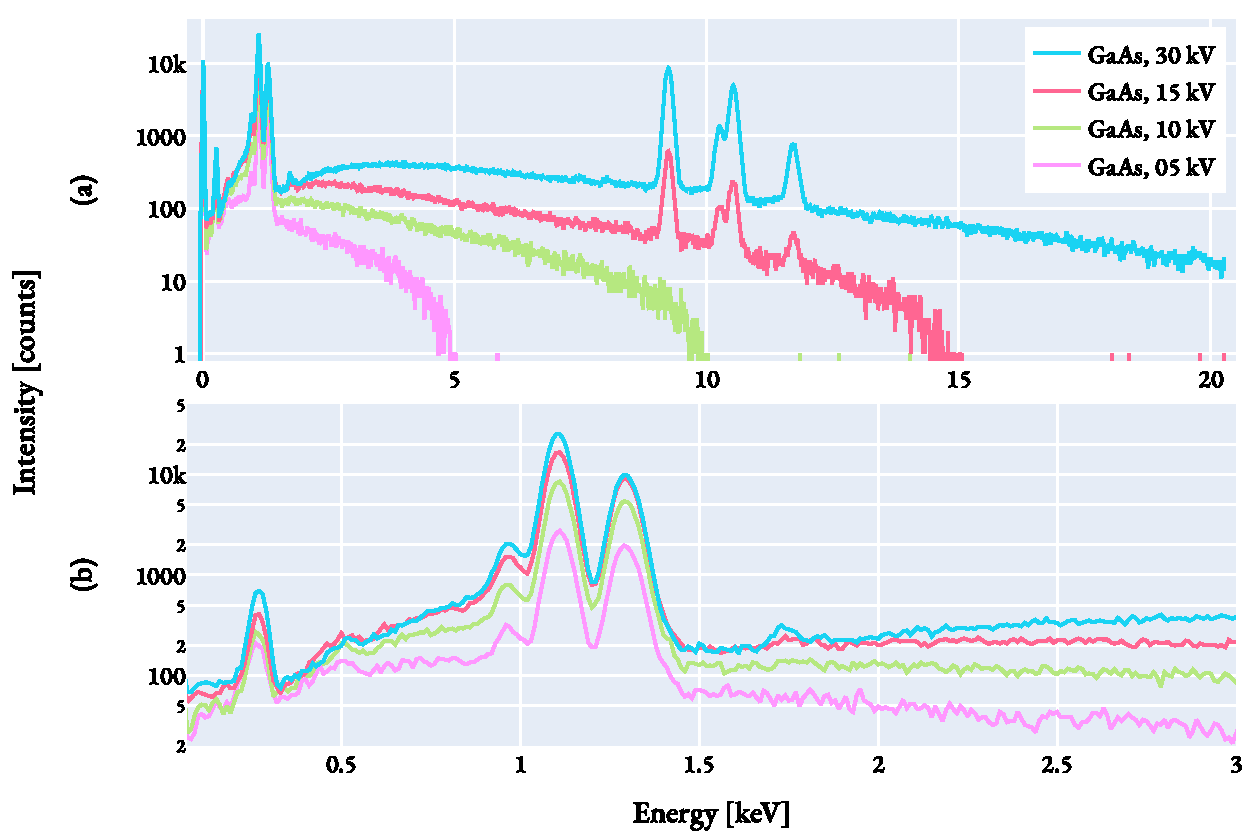
\includegraphics[width=0.85\linewidth]{figures/results/GaAs_voltages.pdf}
    \caption{
        Group (A), the GaAs voltage series.
        The figure gives an overview of the spectra, and show the effect of overvoltage.
        All four spectra have $i_b$ = 25 pA and PT 6.
    }
    \label{fig:results:GaAs_voltages}
\end{figure}


% figures/results/GaSb_voltages.pdf
\begin{figure}[hbtp]
    \centering
    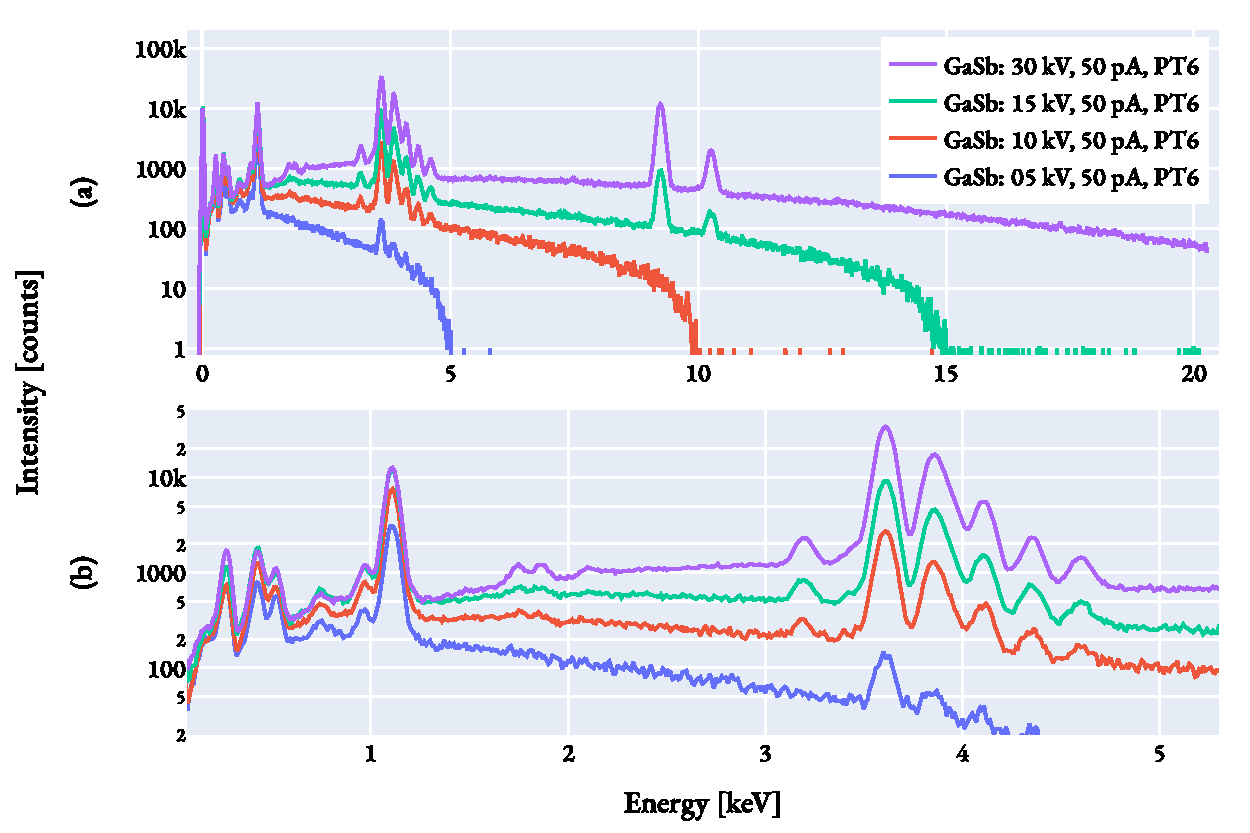
\includegraphics[width=0.85\linewidth]{figures/results/GaSb_voltages.pdf}
    \caption{
        Group (B), the GaSb voltage series.
        The figure serves the same purpose as \cref{fig:results:GaAs_voltages}, but for GaSb.
        % Additionally, an increased amound of coincidence counts compared to the GaAs spectra is visible in the tailing backgrounds, especially at 15 kV.
        The tailing background is the vertical lines above $E_0$.
        All four spectra have $i_b$ = 50 pA and PT 6.
    }
    \label{fig:results:GaSb_voltages}
\end{figure}





% \subsection*{Lines}
% \label{results:qualitative_analysis:lines}

All the lines given in \cref{tab:theory:lineEnergies} for Ga, As, and Sb have been identified in the spectra.
All spectra also had a peak at C K$\alpha$.
% TODO Ton: discus this C_Ka artifact, origin, in discussions
% TODO Ton: No other common peaks like Fe, or Si from set-up?
The GaSb spectra included a well defined O K$\alpha$ peak, while the GaAs spectra had barely any signal from the O K$\alpha$ line.
% TODO discuss: the O Ka peak might also be a Sb M-line, but I have not found the energy of the Sb M-lines.
As annotated in \cref{fig:results:overviewGaSb_withArtifacts}, the GaSb spectra also included two Sb M-signals: $\eta$ and $\gamma$, where $\eta$ is a clearly defined peak, while $\gamma$ is a slight increase in intensity.
These two M-peaks are not listed in the HyperSpy database, but were found through AZtec \cite{aztec_manual} and other literature \cite{liao2006practical}.
% TODO discuss: M lines are present in the absorption plot of GaSb



% \subsection*{Artifacts}
% \label{results:qualitative_analysis:artifacts}

Artifacts are present in all spectra, in varying degrees.
The artifacts identified are listed and described in \cref{tab:results:artifacts}.
The artifacts present in the spectra are the background, the noise peak, the carbon and oxygen stray peak, coincidence peaks, the internal Si fluorescence peak, and the Si escape peak from Sb La.

% The background is present in all spectra, and with increasing background intensity with higher count rates.
% The effect of a strong absorption edge which reduce the background intensity above its energy is most prominent in the GaAs spectra.
% Here it is the absorption edge in the L-peaks which reduce the background intensity abruptly above the L-peaks.
% Coincidence peaks are only present in some spectra, and are most prominent in the spectra with very high count rates.
% The spectra with beam energy 5, 10, and 15 keV also show coincidence events above $E_0$, e.g. visible in panel (a) in \cref{fig:results:GaSb_voltages}.


\begin{table}[phtb]
	\begin{center}
		\caption{
			The artifacts present in the spectra.
			See \cref{fig:results:overviewGaSb_withArtifacts,fig:results:GaSb_voltages,fig:results:GaAs_voltages}.
		}
		\renewcommand*{\arraystretch}{1.4}
		\label{tab:results:artifacts}
		\begin{tabular}{p{3.5cm}p{11.1cm}}
			\hline
			\textbf{Artifact}                                & \textbf{Where the articat is present and a comment}                                                                                                                                                                                                                                                                                                                                                                                             \\
			\hline
			Background                                       & All spectra. Increase with higher count rate.                                                                                                                                                                                                                                                                                                                                                                                                   \\
			Absorption edge effect on background             & Most prominent in GaAs. Reduces the background intensity above the Ga L absorption edge. In \cref{fig:results:GaAs_voltages} panel (b) the background drop from around 600 to around 170 counts.                                                                                                                                                                                                                                                \\
			Noise peak                                       & All spectra. Located almost at 0 keV.                                                                                                                                                                                                                                                                                                                                                                                                           \\
			Coincidence peaks                                & Only the spectra with very high count rates. \cref{fig:results:overviewGaSb_withArtifacts} with GaSb taken at 30 kV, 400 pA, and PT1 show coincidence peaks from: (Sb L + Sb L), (Sb L + Ga K), and (Ga K + Ga K).                                                                                                                                                                                                                              \\
			Tailing background noise from coincidence events & Present in spectra taken at 5, 10, and 15 kV. Coincidence events from two arbitrary counts give a tailing background. Exemplified by the green 15 kV line in \cref{fig:results:GaSb_voltages} panel (a), where vertical lines (one count each) are present between 15 and 20 keV.                                                                                                                                                               \\
			Internal fluorescence peak                       & Visible in some spectra. A low signal, barely a peak in some spectra, at Si K$\alpha$.                                                                                                                                                                                                                                                                                                                                                          \\
			Si escape peak                                   & Most GaSb spectra show some escape signal from Sb L$\alpha$ at 1.86 keV, labeled in \cref{fig:results:overviewGaSb_withArtifacts} panel (b). The coincidence counts from (Sb L + Sb L) marked as "Coincidence 1" in \cref{fig:results:overviewGaSb_withArtifacts} panel (a) has one peak at 7.2 keV and one at 7.5 keV, where the latter cound be a combination of coincidence events and escape counts from Ga K$\alpha$ (9.25 - 1.74 = 7.51). \\
			Stray C                                          & All spectra show a C K$\alpha$ peak, with some variation in intensity.                                                                                                                                                                                                                                                                                                                                                                          \\
			Stray O                                          & All spectra of GaSb show an O K$\alpha$ peak. The GaAs spectra have much lower, but still present signal at 0.52 keV.                                                                                                                                                                                                                                                                                                                           \\
			\hline
		\end{tabular}
	\end{center}
\end{table}



























% 2 setup
\section{Characterization of the setup}
\label{results:setup}

The parameters of the setup are: energy resolution, the energy scale and offset, peak ratios, and deviations in peak positions.
To show how the info in a single spectrum varies with the selected line of reference, information from the lines are presented from two selected spectra in \cref{tab:results:lines_info_30kV_50pA}.
The two selected spectra are both acquired with 30 kV, 50 pA, PT 6, DT 44\%, and ICR = 17k cps for GaSb and ICR = 16.5k cps for GaAs.
The table lists the theoretical energy of the line, the change in position after calibration, the FWHM of the peak, the area of the peak, the Fiori P/B of the line, and the estimated FWHM of Mn K$\alpha$ using \cref{eq:estimateFWHM}.


\begin{table}[phtb]
    \begin{center}
        \caption{
            Info from the lines acquired at 30 keV, 50 pA, and PT 6.
            The lines are sorted by area (counts in the peak).
            %The table lists the theoretical energy of the line, the change in position after calibration, the FWHM of the peak, the area of the peak, the Fiori P/B of the line, and the estimated FWHM of Mn K$\alpha$ using \cref{eq:estimateFWHM}.
            Both the GaAs and GaSb spectra have DT 44\%, with ICR = 17k cps for GaSb and ICR = 16.5k cps for GaAs.
        }
        \renewcommand*{\arraystretch}{1.4}
        \label{tab:results:lines_info_30kV_50pA}
        \begin{tabular}{llrlrrrp{2.5cm}}
            \hline
            \textbf{Specimen} & \textbf{Line} & \textbf{Energy} & \textbf{$\Delta$ E} & \textbf{FWHM} & \textbf{Area}     & \textbf{Fiori P/B} & \textbf{Estimated FWHM(Mn K$\alpha$)} \\
                              &               & \emph{[keV]}    & \emph{[eV]}         & \emph{[eV]}   & \emph{[k counts]} &                    & \emph{[eV]}                           \\
            \hline
                              & Ga L$\alpha$  & 1.098           & 2                   & 67            & 333               & 586                & 128                                   \\
                              & Ga K$\alpha$  & 9.252           & 2                   & 163           & 302               & 762                & 134                                   \\
                              & As K$\alpha$  & 10.544          & 2                   & 173           & 183               & 622                & 135                                   \\
            GaAs              & As L$\alpha$  & 1.282           & 2                   & 72            & 140               & 236                & 129                                   \\
                              & Ga L$\beta$   & 1.125           & 0                   & 68            & 56                & 97                 & 129                                   \\
                              & Ga K$\beta$   & 10.264          & 2                   & 161           & 39                & 124                & 123                                   \\
                              & As K$\beta$   & 11.726          & 2                   & 181           & 27                & 117                & 135                                   \\
                              & As L$\beta$   & 1.317           & 0                   & 71            & 23                & 39                 & 129                                   \\
            \hline
                              & Sb L$\alpha$  & 3.605           & -0.4                & 102           & 355               & 385                & 127                                   \\
                              & Ga K$\alpha$  & 9.252           & -2                  & 161           & 189               & 408                & 133                                   \\
            GaSb              & Sb L$\beta_1$  & 3.844           & -2                  & 101           & 152               & 168                & 124                                   \\
                              & Ga L$\alpha$  & 1.098           & 2                   & 65            & 74                & 86                 & 128                                   \\
                              & Sb L$\beta_2$  & 4.101           & 0                   & 108           & 55                & 63                 & 127                                   \\
                              & Ga K$\beta$   & 10.264          & -2                  & 160           & 24                & 59                 & 121                                   \\
            %&&&&&&&\\
            \hline
        \end{tabular}
    \end{center}
\end{table}



\subsection*{Energy resolution of the detector}
\label{results:setup:energy_resolution}

The energy resolution, as the estimated FWHM of the Mn K$\alpha$ peak, is both a function of the detector and certain acquisition parameters.
In the GaSb spectra the best energy resolution was 124 eV, obtained with PT 6, ICR = 22k cps, $E_0$ = 15 kV, and $i_b$ = 200 pA.
In the GaAs spectra the best energy resolution was 127 eV, obtained with PT 6, ICR = 880 cps, $E_0$ = 5 kV, and $i_b$ = 25 pA.
% TODO discuss: no obvious relation between the two best energy resolutions. But, it depends on the peaks in the spectrum.
% The best energy resolution obtained was: 124 eV for the GaSb spectra with PT 6, and 127 eV for the GaAs spectra.
The energy resolution should not be a function of the specimen, but as it is calculated with \cref{eq:estimateFWHM}, the outputted number depends somewhat on the peaks in the spectrum.
This is shown in \cref{tab:results:lines_info_30kV_50pA}, where the highest and lowest estimated energy resolution is 123 eV and 135 in the GaAs spectrum, and 121 eV and 133 eV in the GaSb spectrum.
% TODO discuss: Different peaks are used in GaSb and GaAs, thus we get different number with equal acquisition parameters.
% TODO discuss: Ga Kb gives the lowest, which might be a result of the overlap with As Ka.
The energy resolutions for all spectra are listed in \cref{tab:results:energy_resolutions}, with the relevant acquisition parameters.
These numbers for the energy resolution is calculated with HyperSpy, which have an issue explained in \cref{theory:eds_performance:energyres}.
As \cref{tab:results:energy_resolutions} shows, the energy resolution is affected by the two acquisition parameters: (i) process time and (ii) input count rate.
The ICR change with $E_0$ and $i_b$.
Specifying a single energy resolution for the detector should be accompanied by the acquisition parameters used to obtain that energy resolution.
Preferably, the value should also be an average with an uncertainty, calculated by several measurements with equal acquisition parameters.
This is not done here, but the values in \cref{tab:results:energy_resolutions} show that PT 6 give the best energy resolution at about 127 $\pm$ 2 eV.
When \cref{tab:results:lines_info_30kV_50pA} with the variations based on the peak of reference is taken into account, the energy resolution is more like 127 $\pm$ 6 eV.
% TODO discuss: The energy resolution is more like +- 6 eV, when we take into account the variations when using different peaks.



\begin{table}[htbp]
    \begin{center}
        \caption{
            The energy resolutions [eV] in the different spectra.
            The table is sorted by process time, then ICR.
            All energy resolutions are calculated with \cref{eq:estimateFWHM}.
        }
        % \renewcommand*{\arraystretch}{1.4}
        \label{tab:results:energy_resolutions}
        \begin{tabular}	{p{1.5cm}ccrrr}
            \hline
            \textbf{		} & \textbf{	Energy resolution	} & \textbf{	PT	} & \textbf{	ICR	} & \textbf{	E$_0$	} & \textbf{	I$_\textnormal{beam}$	} \\
            \hline
                        & 158                          & 1             & 17000          & 30               & 50                               \\
                        & 158                          & 1             & 160000         & 30               & 400                              \\
                        & 143                          & 2             & 17000          & 30               & 50                               \\
                        & 132                          & 4             & 17000          & 30               & 50                               \\
                        & 128                          & 6             & 1080           & 5                & 50                               \\
            GaSb        & 127                          & 6             & 2300           & 10               & 50                               \\
                        & 125                          & 6             & 5700           & 15               & 50                               \\
                        & 127                          & 6             & 17000          & 30               & 50                               \\
                        & 127                          & 6             & 17000          & 30               & 50                               \\
                        & 124                          & 6             & 22000          & 15               & 200                              \\
                        & 125                          & 6             & 42000          & 15               & 400                              \\
            \hline
                        & 127                          & 6             & 880            & 5                & 25                               \\
                        & 127                          & 6             & 1750           & 10               & 25                               \\
            GaAs        & 129                          & 6             & 3300           & 15               & 25                               \\
                        & 128                          & 6             & 8000           & 30               & 25                               \\
                        & 129                          & 6             & 16400          & 30               & 50                               \\
            \hline
        \end{tabular}
    \end{center}
\end{table}



\subsection*{Energy scale and offset}
\label{results:setup:scale_offset}

The energy scale and offset are the parameters which are used to calibrate the spectra.
Both metrics are quite consistent between the spectra, and the energy scale match with the setting used in the acquisition (10 eV per channel).
The averaged values and the standard deviations are listed in \cref{tab:results:scale_offset}.
The calculated scale of the detector is equal to the instrument setting at 10 eV per channel, with very low standard deviation between the spectra at 0.04 eV/channel.
The zero offset was calculated to be -0.205 keV, which is a deviation of half a channel from the instrument setting of -0.2 keV.
The standard deviation of the offset is 0.004 keV.

% TODO discuss: Comment that the std of the offset is one order of magnitude closer to the avg compared to the std vs avg of the scale.
% TODO discuss: why GaSb is slightly better std, might be because of the lines but also the higher i_b which gives more counts.

\begin{table}[htbp]
    \begin{center}
        \caption{
            The scale and offset in the spectra.
        }
        \renewcommand*{\arraystretch}{1.2}
        \label{tab:results:scale_offset}
        \begin{tabular}{rrrrr}
            \hline
            \textbf{Samples}   & \textbf{Scale, average} & \textbf{Scale, std}  & \textbf{Offset, average} & \textbf{Offset, std} \\
                               & \emph{[keV/channel]}    & \emph{[keV/channel]} & \emph{[keV]}             & \emph{[keV]}         \\
            \hline
            Instrument setting & 0.010000                & -                    & -0.2000                  & -                    \\

            GaSb               & 0.010001                & 8.7E-06              & -0.2044                  & 4.4E-03              \\
            GaAs               & 0.010018                & 6.6E-05              & -0.2075                  & 4.9E-03              \\
            GaSb + GaAs        & 0.010007                & 3.8E-05              & -0.2054                  & 4.3E-03              \\
            \hline
        \end{tabular}
    \end{center}
\end{table}




\subsection*{Peak ratios}
\label{results:setup:peak_ratios}

The results from the peak ratios are listed in \cref{tab:results:peak_ratios}.
The peak ratios are useful to alert carbon contamination over time, and to identify and quantify stray radiation with certain sample geometry.
As the results are neither a series over time or taken with the required sample geometry, the results in the table are a demonstration of the metric without any further interpretation.
Peak ratios are also used for quantification, but needs bulk corrections.
The table show that some of the peak ratios vary greatly with the acquisition parameters, e.g. the ratio between Ga L$\alpha$ and Sb L$\alpha$.


\begin{table}[phtb]
    \begin{center}
        \caption{
            Peak ratios calculated.
            The values varies with the beam energy, and thus the beam energies are grouped and an average is given with the corresponding standard deviation.
        }
        \renewcommand*{\arraystretch}{1.4}
        \label{tab:results:peak_ratios}
        \begin{tabular}{ccccl}
            \hline
            \textbf{Peaks}               & \textbf{$E_0$} & \textbf{Peak ratio} & \textbf{STD} & \textbf{Comment}              \\
            \hline
            Sb L$\alpha$ / Sb L$\beta_1$ & All            & 2.34                & 0            & Equal for all 11 GaSb spectra \\
            Ga L$\alpha$ / Sb L$\alpha$  & 5 kV           & 33.31               & -            & 1 GaSb spectrum               \\
            "                            & 10 kV          & 1.73                & -            & 1 GaSb spectra                \\
            "                            & 15 kV          & 0.76                & 0.008        & 3 GaSb spectra                \\
            "                            & 30 kV          & 0.21                & 0.004        & 6 GaSb spectra                \\
            Ga K$\alpha$ / Ga L$\alpha$  & 15 kV          & 0.19                & 0.0005       & 3 GaSb spectra                \\
            "                            & 15 kV          & 0.07                & -            & 1 GaAs spectrum               \\
            "                            & 30 kV          & 2.61                & 0.06         & 6 GaSb spectra                \\
            "                            & 30 kV          & 0.90                & 0.005        & 2 GaAs spectra                \\
            \hline
        \end{tabular}
    \end{center}
\end{table}



\brynjar{Eventually, take a new set of data to look at carbon contamination over time. Then make the table.}

\brynjar{TODO: redo these results. From ton: "yes, think is good to do. What
    would the advice be at the end? Take series or compare ratios for first and last
    spectrum to exclude C-contamination? For discussion: How does the measured ratio
    compare to the theoretical (quantum mechanics) ratio? And why?"}



\subsection*{Deviations in peak positions}
\label{results:setup:peak_positions}

No significant deviations in peak positions were observed.
The maximum deviation was 2 eV, and the minimum deviation was -2 eV, which is very low compared to the energy of the lines which are > 1 keV.



















% 3
\section{Optimization of the acquisition parameters}
\label{results:acquisition_parameters}

The performance metrics of the acquisition are: the Duane-Hunt limit, the Fiori peak-to-background ratio, and portion of counts in peaks vs background.
Additionally, results from selected user parameters are presented, such as the process time, beam energy, and beam current.
The energy resolution is affected by both the detector and the acquisition setup, and the relevant results are presented in \cref{results:setup:energy_resolution}.



\subsection{Process time}
\label{results:process_time}

One of the parameters which was tested was the process time.
The process time is a trade-off between the energy resolution and the throughput.
This effect is illustrated in \cref{fig:results:energy_resolutions_process_time}, which is a plot of the GaSb spectrum at minimum and maximum process time.
Both spectra are taken at 30 kV with 50 pA.
The figure have three panels, (a) for low, (b) for medium, and (c) for high energy X-rays.
The effect of the lowered energy resolution is most prominent for the low energy X-rays.
The difference between the observable center of the peaks and the theoretical line energies in panel (a) is due to the poorer calibration at sub 1 keV energies.
In panel (a), the Sb M$\eta$ and O K$\alpha$ are merged together with PT 1, but are separated with PT 6.
The ability to seperate peaks is the definition of energy resolution, thus panel (a) is a good illustration of different energy resolutions.
The Ga L$l$ and Ga L$\alpha$ peaks are seperated with PT 6, but are merged together with PT 1.
With PT 4 (not shown), the Ga L$l$ and Ga L$\alpha$ peaks still seperated, but with PT 2 (not shown) they are merged together.
% TODO discuss: visible seperable and seperable with gaussian modelling is different. Visible seperable is important for qualitative analysis. And the quantitative is probably better with more seperated peaks, but overlapping can be dealt with quire well.
\cref{tab:results:energy_resolutions} show that the energy resolution with PT 1 is 158 eV, and with PT6 it is 127 eV.
In panel (b) with the medium energies, the contrast of the peaks are lowered, i.e. the difference between the top of the peaks and the valley between the peaks are lowered.
The effect of the lowered energy resolution is not as prominent panel (c) for high energy X-rays.

% TODO discuss: for high energies the peaks are also well seperated.


% figures eds_energyResolutions_process_time.pdf
\begin{figure}[hptb]
    \centering
    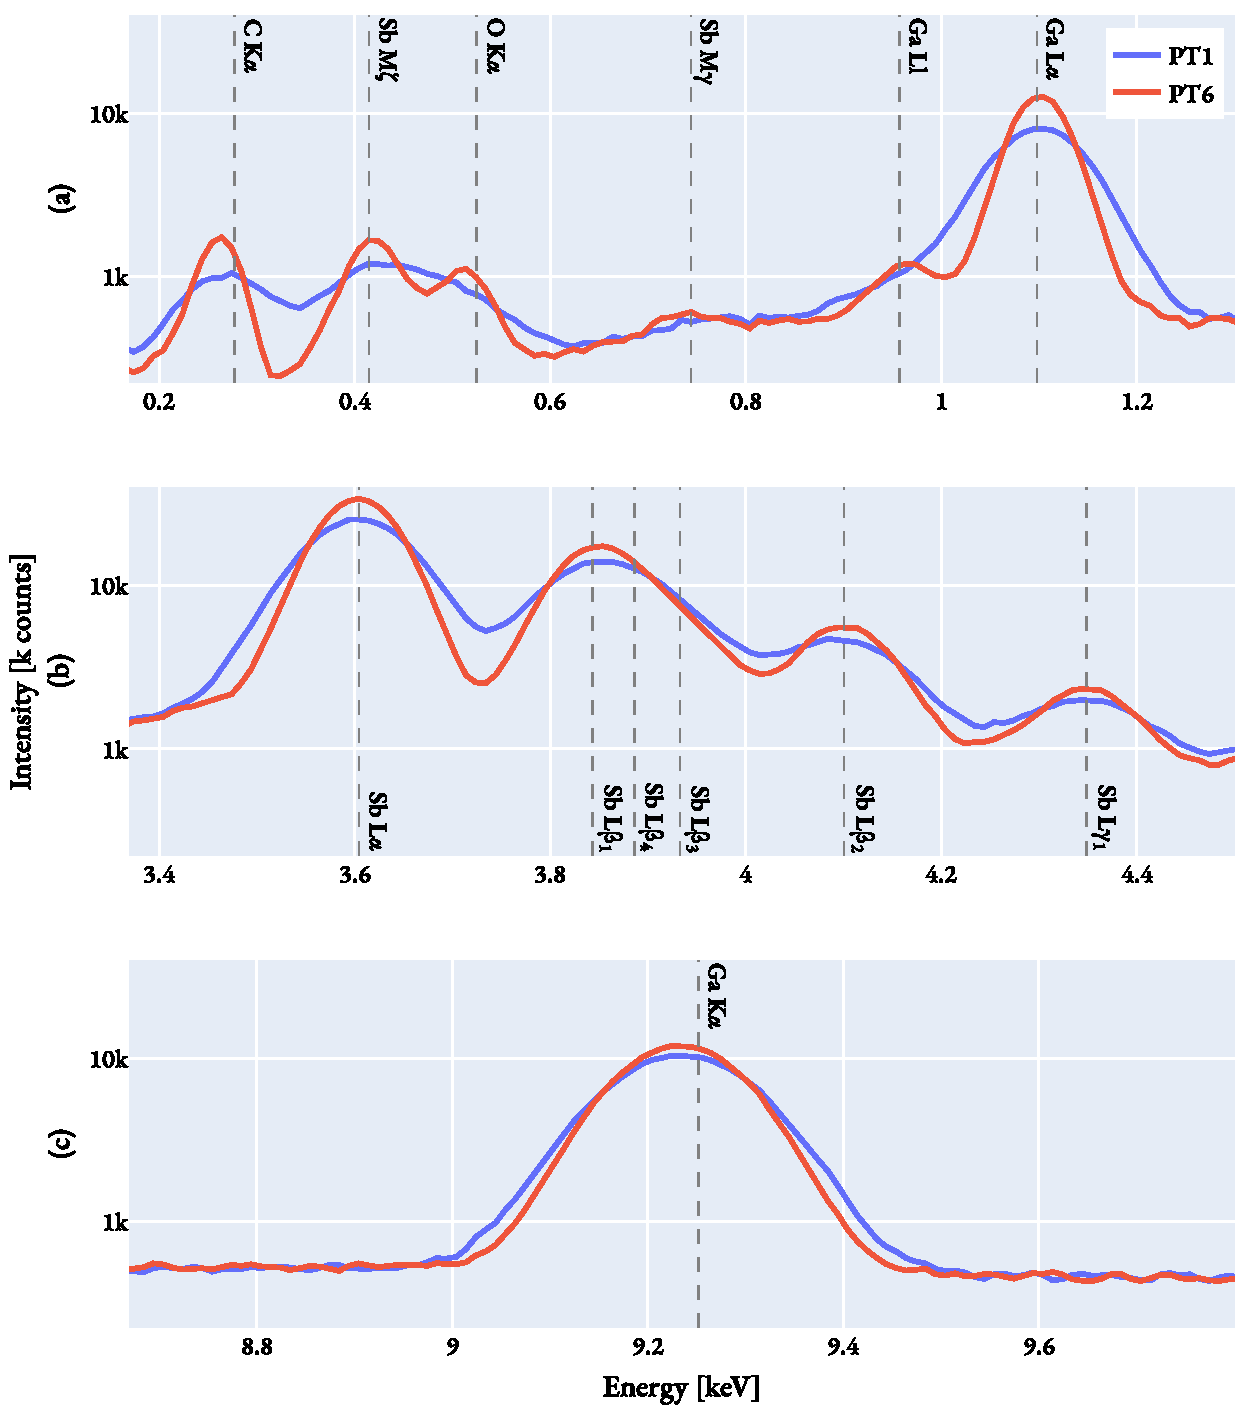
\includegraphics[width=0.95\linewidth]{figures/results/eds_energyResolutions_process_time.pdf}
    \caption{
        Different energy resolutions on the same specimen, because of different process times.
        The maximum (red) and minimum (blue) PT on the instrument is used.
        $E_0$ = 30 kV, $I_b$ = 50 pA for both spectra.
        The PT 1 and PT 4 spectra are not shown, but are in between the PT 2 and PT 6 spectra.
        Panel (a) is the spectrum at low energy, where the effect most influential.
        With PT 1 the Sb M$\eta$ and O K$\alpha$ peak are merged, and the Ga L$l$ and Ga L$\alpha$ peaks are merged.
        Panel (b) is the spectrum at medium energy, where the effect less influential, but the peak contrast is lowered.
        Panel (c) is the spectrum at high energy, where the effect is almost negligible.
        All three panels span 1.13 keV and have the same range of counts.
        The vertical lines are the theoretical line energies.
    }
    \label{fig:results:energy_resolutions_process_time}
\end{figure}


The effect of the process time on the FWHM of the lines is shown in \cref{tab:results:PTvsFWHMs}.
The table shows the measured FWHM of Ga L$\alpha$, Sb L$\alpha$, and Ga K$\alpha$ for different process times.
The measurement is done on the Gaussian fit of the peaks.
Additionally, the FWHM of the Mn K$\alpha$ is estimated for each process time.
The table shows the variations on the GaSb specimen with PT 1, 2, 4, and 6.
The last row shows the FWHM in the GaAs specimen at PT 6 for reference.
All spectra in the table were acquired at 30 kV and 50 pA.
In the GaSb spectra, the PT 1 has DT 4\%, PT 2 has DT 7\%, PT 4 has DT 13\%, and PT 6 has DT 44\%. 
The GaAs spectrum with PT 6 has DT 44\%.

% TODO discuss: based on the numbers, PT 4 should be good enough for most applications. High resolution, and much faster than PT 6. DT44 is really high, and not nice for mapping.
% TODO discuss: specimen with many L-lines


\begin{table}[phtb]
    \begin{center}
        \caption{
            FWHMs of lines with different process times.
            All the FWHMs are in eV, calculated from the Gaussian fit.
            All spectra are acquired at 30 kV and 50 pA.
            GaSb is used as the specimen, except for the last column, where GaAs is used for reference.
        }
        \renewcommand*{\arraystretch}{1.4}
        \label{tab:results:PTvsFWHMs}
        \begin{tabular}{rrrrrr}
            \hline
            \textbf{Line}       & \textbf{PT 1} & \textbf{PT 2} & \textbf{PT 4} & \textbf{PT 6} & \textbf{PT 6, GaAs} \\
            \hline
            %C K$\alpha$&&&&&\\ % C is not it the models used
            Ga L$\alpha$        & 109           & 88            & 73            & 65            & 67                  \\
            Sb L$\alpha$        & 138           & 122           & 108           & 102           & -                   \\
            Mn K$\alpha$ (est.) & 158           & 143           & 132           & 127           & 129                 \\
            Ga K$\alpha$        & 182           & 172           & 165           & 161           & 163                 \\
            \hline
        \end{tabular}
    \end{center}
\end{table}






\clearpage

% 4.4
\section{Quantitative analysis}
\label{results:quantitative}


\brynjar{Coming soon. I do observations of AZtec, try out HyperSpy, and make new code which are a step in the right direction (e.g. XPP in a notebook, which is concrete and quantitative.)}


\subsection{Initial quantification}
\label{results:initial_quantification}

% initial quantification (AZtec and i/i_sum)
Initial quantification was done with the AZtec software.
Then quantification was done without any corrections, where the area in P1 (peak one) is divided by the sum of area in P1 and P2.
P1 and P2 was chosen as the two most similar peaks, i.e. two L$\alpha$ or two K$\alpha$ when possible.
These results from selected spectra are shown in \cref{tab:results:initial_quantification}.
As the table shows, some of the results are close to 50\%.
AZtec is mostly at 50$\pm$ 2\%, while the composition from the area without corrections is more spread out.
The uncorrected results from the GaSb spectra with $E_0$ = 30 kV are at 50$\pm$ 2\%.
The 15 kV results from GaSb have a deviation of $\pm$ 10\%.
The low energy results from GaAs have a high deviation, probably due to issues with overvoltage.
The GaAs results are deviating more, implying a need for corrections.



% TODO discuss: AZtec is pretty good, but misses at eg 5kV GaSb
% TODO discuss: the uncorrected results are good for some spectra, but others are bad. Overvoltage might be the main reason.
% TODO discuss: also comparing Ga Ka with Sb La, which should have different omega (ref to image in theory)
% TODO discuss: bulk corrections is needed

\begin{table}[phtb]
    \begin{center}
        \caption{
            Initial quantification in selected spectra.
            Composition from Aztec and the relative composition by taking the area in the peak and divide it by the summed area of the two peaks, and coverting the wt\% to at\%.
        }
        %\renewcommand*{\arraystretch}{1.4}
        \label{tab:results:initial_quantification}
        \begin{tabular}{rrrrrrrr}
            \hline
            \textbf{ Group} & \textbf{Line used} & \textbf{$E_0$} & \textbf{$i_b$} & \textbf{PT} & \textbf{Area}     & \textbf{AZtec comp.} & \textbf{Comp. area/sum(area)} \\
            \emph{}         & \emph{}            & \emph{[kV]}    & \emph{[pA]}    & \emph{}     & \emph{[k counts]} & \emph{[at\%]}        & \emph{[at\%]}                 \\
            \hline
            A               & As L$\alpha$       & 5              & 25             & 6           & 13                & 53.4                 & 42.7                          \\
            A               & Ga L$\alpha$       & 5              & 25             & 6           & 16                & 46.6                 & 57.3                          \\
            A               & Ga L$\alpha$       & 10             & 25             & 6           & 51                & 48.1                 & 60.0                          \\
            A               & As L$\alpha$       & 10             & 25             & 6           & 37                & 51.9                 & 40.0                          \\
            A               & As L$\alpha$       & 15             & 25             & 6           & 62                & 50.6                 & 35.7                          \\
            A               & Ga L$\alpha$       & 15             & 25             & 6           & 103               & 49.4                 & 64.3                          \\
            A               & As K$\alpha$       & 30             & 25             & 6           & 84                & 48.4                 & 35.6                          \\
            A               & Ga K$\alpha$       & 30             & 25             & 6           & 141               & 51.6                 & 64.4                          \\
            A               & As K$\alpha$       & 30             & 50             & 6           & 180               & 48.3                 & 35.5                          \\
            A               & Ga K$\alpha$       & 30             & 50             & 6           & 303               & 51.7                 & 64.5                          \\
            \hline
            B               & Ga L$\alpha$       & 5              & 50             & 6           & 19                & 39.0                 & 97.1                          \\
            B               & Sb L$\alpha$       & 5              & 50             & 6           & 1                 & 61.0                 & 2.9                           \\
            B               & Ga L$\alpha$       & 10             & 50             & 6           & 46                & 46.8                 & 74.8                          \\
            B               & Sb L$\alpha$       & 10             & 50             & 6           & 27                & 53.2                 & 25.2                          \\
            B               & Ga L$\alpha$       & 15             & 50             & 6           & 74                & 49.1                 & 58.0                          \\
            B               & Sb L$\alpha$       & 15             & 50             & 6           & 94                & 50.9                 & 42.0                          \\
            B               & Ga K$\alpha$       & 30             & 50             & 6           & 191               & 50.2                 & 48.1                          \\
            B               & Sb L$\alpha$       & 30             & 50             & 6           & 359               & 49.8                 & 51.9                          \\
            \hline
            C               & Ga K$\alpha$       & 30             & 50             & 4           & 189               & 50.2                 & 48.5                          \\
            C               & Sb L$\alpha$       & 30             & 50             & 4           & 350               & 49.8                 & 51.5                          \\
            C               & Ga K$\alpha$       & 30             & 50             & 2           & 184               & 50.2                 & 49.3                          \\
            C               & Sb L$\alpha$       & 30             & 50             & 2           & 330               & 49.8                 & 50.7                          \\
            C               & Ga K$\alpha$       & 30             & 50             & 1           & 178               & 50.4                 & 50.5                          \\
            C               & Sb L$\alpha$       & 30             & 50             & 1           & 304               & 49.7                 & 49.5                          \\
            \hline
            D               & Ga K$\alpha$       & 30             & 400            & 1           & 1724              & 50.0                 & 50.1                          \\
            D               & Sb L$\alpha$       & 30             & 400            & 1           & 2996              & 50.0                 & 49.9                          \\
            D               & Ga L$\alpha$       & 15             & 200            & 6           & 155               & 48.7                 & 57.4                          \\
            D               & Sb L$\alpha$       & 15             & 200            & 6           & 200               & 51.3                 & 42.6                          \\
            D               & Ga L$\alpha$       & 15             & 400            & 6           & 284               & 48.7                 & 57.4                          \\
            D               & Sb L$\alpha$       & 15             & 400            & 6           & 367               & 51.3                 & 42.6                          \\
            % \hline
            % E               & Map                &                &                &             &                   &                      &                               \\
            % E               & Map                &                &                &             &                   &                      &                               \\
            % &&&&&&&\\
            \hline
        \end{tabular}
    \end{center}
\end{table}



\subsubsection*{Quantification of SEM data, pretended to be TEM data}

% Quantification while treating the specimen as a TEM specimen.
Quantification of the spectra was also done pretending that the specimen was a TEM specimen, both in AZtec and HyperSpy.
This is done in AZtec with the "TEM setting", which gives composition and calculated k-factors.
The calculated k-factors were taken and used with the Cliff-Lorimer method in HyperSpy, which gives composition.
In HyperSpy, the quantification was done with and without the TEM absorption corrections.
For the absorption corrections, four different thicknesses were used: 100nm, 1000 nm, 10000 nm, and 100000 nm.
As the results were poor, they are only commented on briefly in the text below.

% AZtec TEM setting
The AZtec TEM setting results on the SEM specimen yielded poor results.
The 5 kV GaAs spectrum and the 30 kV GaSb spectra was quantified at a 45:55 ratio.
The remaining spectra were quantified around a 70:30 ratio.


% HyperSpy Cliff-Lorimer
The Cliff-Lorimer TEM quantification method in HyperSpy yielded poor results too.
Adding absorption corrections through the Cliff-Lorimer method did not improve the results.
The implemented absorption correction is a part of the Cliff-Lorimer method, and thus made for TEM specimens.
The low voltage spectra were quantified at a 70:30 ratio or worse.
% todo discuss: probably due to TEM being high HT.
The 30 kV spectra were quantified at a 55-60:45-40 ratio, and the absorption corrections improved the results somewhat with t = 1000 nm for GaSb and t = 10000 nm for GaAs.
% todo discuss: the absorption corrections in the CL method, as used briefly in this work, does not give a general improvement.




\subsection{Matrix corrections}
\label{results:matrix_corrections}



\subsubsection{ZAF absorption corrections}
\label{results:matrix_corrections:ZAF}



\subsubsection{XPP/PAP corrections}
\label{results:matrix_corrections:XPP}



% Old
% % % The model lines

\begin{table}[p]
    \centering
    \caption{
        The lines in the HyperSpy models for the GaAs sample, when As and Ga are added as elements.
        The dashed lines are the lines that are not used in the model, because of low overvoltage.
        HyperSpy differentiates between "X-ray lines" and "Family lines", where the first are the alpha lines of the element.
    }
    \label{tab:results:model_lines}
    \begin{tabular}{c|ccccccccccc}
        X-ray lines  &       &        &       &       &        &       &        &       &       &        \\
        % Model        &       &        &       &       &        &       &        &       &       &        \\
        30 kV        & As Ka & As La  & Ga Ka & Ga La &        &       &        &       &       &        \\
        15 kV        & As Ka & As La  & Ga Ka & Ga La &        &       &        &       &       &        \\
        10 kV        & ----- & As La  & Ga Ka & Ga La &        &       &        &       &       &        \\
        5            & ----- & As La  & ----- & Ga La &        &       &        &       &       &        \\
        \hline
        Family lines &       &        &       &       &        &       &        &       &       &        \\
        30 kV        & As Kb & As Lb1 & As Ln & As Ll & As Lb3 & Ga Kb & Ga Lb1 & Ga Ln & Ga Ll & Ga Lb3 \\
        15 kV        & As Kb & As Lb1 & As Ln & As Ll & As Lb3 & Ga Kb & Ga Lb1 & Ga Ln & Ga Ll & Ga Lb3 \\
        10 kV        & ----- & As Lb1 & As Ln & As Ll & As Lb3 & ----- & Ga Lb1 & Ga Ln & Ga Ll & Ga Lb3 \\
        5  kV        & ----- & As Lb1 & As Ln & As Ll & As Lb3 & ----- & Ga Lb1 & Ga Ln & Ga Ll & Ga Lb3
    \end{tabular}
\end{table}
% \begin{table}[p]
    \centering
    \caption{
        The estimated FWHM of Mn K$\alpha$ with different reference lines.
        When using 'all\_alpha', the alphabetically first line is used as reference.
        That is, for 30 and 15 kV, As K$\alpha$ is used as reference.
        For 10 and 5 kV, As L$\alpha$ is used as reference.
        The original resolution is from the instrument software.
    }
    \label{tab:results:estimated-FWHM}
    \begin{tabular}{ccccc}
        Reference line      & 30 kV & 15 kV & 10 kV & 5 kV  \\
        \hline
        original resolution & 130.0 & 130.0 & 130.0 & 130.0 \\
        \verb|'all_alpha'|  & 138.3 & 148.8 & 132.0 & 132.2 \\
        As Ka               & 137.9 & 146.4 & nan   & nan   \\
        As La               & 130.0 & 130.4 & 131.9 & 132.1 \\
        Ga Ka               & 132.9 & 131.7 & 668.3 & nan   \\
        Ga La               & 129.7 & 130.9 & 127.4 & 130.8
    \end{tabular}
\end{table}
% \subsection{Energy resolution}
% \label{results:resolution}